\documentclass[twocolumn]{aastex62}
\usepackage{amsmath}
\usepackage{natbib}
\usepackage{mhchem}
\bibliographystyle{apj}
\begin{document}
	\title{Chemical impacts of X-ray from an active supermassive black hole in our galaxy}
	\author{Chang Liu}
	\affiliation{Department of Astronomy, Peking University}
	\begin{abstract}
		This is an abstract...
	\end{abstract}
	\keywords{Sgr A*, X-ray, Prebiotic Molecules}
	\section{Introduction}
	
	Supermassive black holes (SMBHs) are widely held in galaxies. The bright radio object Sagittarius A* (Sgr A*) located in the galactic center 8 kpc away from earth is believed as the SMBH in our galaxy. It weighs 
	$4\times10^{6}M_\odot$ and is quite faint with surprisingly low luminosity $L\sim10^{33-35}\text{erg s}^{-1}$. This is no more 
	than $10^{-9}L_{\text{Edd}}$, where $L_{\mathrm{Edd}} \approx 1.3 \times 10^{38}\left(M_{\mathrm{BH}} / M_{\odot}\right) \text{erg} 
	\mathrm{s}^{-1}\sim 5\times10^{44} \text{erg} \mathrm{s}^{-1}$ is the Eddington luminosity \citep{Sabha2010}, showing that Sgr A* is on quiescent state. 
	
	More recent researches challenge the conventional understanding of Observations have shown evidence that Sgr A* went through an active phase 6 million years ago \citep{Nicastro2016}. Activation of Sgr A* triggers radiation of hard X-ray photons. For a hydrogen atom, the photo-ionization cross section $\sigma_p^{\ce{H}}$ is proportional to $(h\nu)^{-3}$ \citep{Brown1970}, where $\nu$ is the frequency of the photon, indicating tiny cross sections with high energetic photons. Hard X-ray photons can therefore transmit much farther than optical and UV photons in galactic disk. \cite{Amaro-Seoane2014} calculated the X-ray irradiation from Sgr A* due to accretion of gas (like an AGN) and the tidal disruption, Sgr A* could precipitate on Earth a hard X-ray (i.e. $h\nu > 2$ keV) flux comparable to that from the current quiescent sun, while UV and soft X-ray photons suffer from heavy extinction and are not significant 8 kpc away from galactic center. These energetic photons may leave significant physical and chemical records in molecular gas around galactic center \citep{Krolik1983, Neufeld1994, Aalto2014} and planetary atmospheres \citep{Loeb2018,Wis2019}.
	In our case, we focus on the chemical evolution in dense molecular clouds under the X-ray radiation of an active Sgr A*. 
	\section{Methods}
	\subsection{X-ray flux in different distances from Sgr A*}
	\subsection{X-ray chemistry}
	Energetic hard X-ray photons cause various physical and chemical effects in a molecular cloud. X-ray photon with energy of $\sim 1\text{ keV}$ can directly ionize $\ce{H,He}$ and heavier atoms. The rapid electrons emitted by direct ionization or Auger process, which is known as primary electrons, influence the system by
	(i) Ionizing more atoms through collisions which leads to the emission of secondary electrons \citep{Shull1985,Krolik1983,Maloney1996};
	(ii) X-ray heating through Coulomb scattering with ambient thermal electrons;
	(iii) Excitation of various atomic and molecular species;
	(iv) FUV photon flux induced by collisions with hydrogen atoms. 
	The energy deposition of each branch depends on the ionization fraction $x_e=n_e/n_{\ce{H}_{tot}}$, which is ratio of the number density of free electrons and the total hydrogen number density $n_{\ce{H}}=n({\ce{H}})+2n({\ce{H2}})$.
	
	The most direct and profound chemical effects come from direct and secondary photoionization,  which produces reactive ions and radicals (species with unpaired electrons and thus unstable) \citep{Herbst1973, Herbst2009}. In cold cores where the temperature is too low ($T\sim10\text{ K}$) to trigger off any reaction with high energy barrier, the reaction between stable neutral species, which typically have high activation energy, are much slower and less efficient than ion-molecular and radical reactions \citep{Herbst1973, Wakelam2010}. Therefore ionization processes are necessary for the synthesis of more complex molecules, including prebiotic organic species which we are mostly interested in.
	
	Other X-ray processes above mainly induce thermal effects and enhance the gas temperature, which also influence the rates of many reactions. By introducing heating processes, the temperature of the system becomes time-dependent in an AGN event. For high ionized interstellar mediums, X-ray heating is rather efficient because of high number density of thermal electrons. But for the neutral environment we consider (low ionization fraction $x_e$), although the fraction of energy of X-ray flux goes to the ambient thermal electrons and deposited as heat is still considerable, the free electrons are too scarce to cause significant Coulomb scattering. In this way, in our simplified models, we assume an empirical, time-independent temperature and consider only the effect caused by (primary and secondary) ionization. For future work, heating processes should be taken into account to study the effects of X-ray more thoroughly.
	\subsubsection{Primary ionization}
The physical and chemical state of the dense cloud is insensitive to the shape of the X-ray spectrum, but depends on the energy deposition on different procedures \citep{Maloney1996}. When considering specifically the photoionization, the primary ionization rate for species $i$ is \citep{Latif2015}
\begin{equation}
\label{eq:1}
\zeta_p^i=\int_{E_{min}}^{E_{max}}\frac{F(E)}{E}e^{-\tau(E)}\sigma^i(E)\text{d}E \quad \left[ \mathrm { s } ^ { - 1 } \right]
\end{equation}
where $F$ is the monochromatic flux of X-ray at the edge of the molecular cloud, $\tau$ is the optical depth of the cloud and $\sigma^i$ is the cross section of photoionization of species $i$ taken from \cite{Verner1996}. 

To estimate the optical depth, we take Jeans length as the size of the cloud
$$
\lambda_J=\sqrt{\frac{\pi kT}{G\rho \mu m_p}}
$$
where $\rho$ is the mass density of the cloud, $m_p$ is the mass of a proton and $\mu$ is the (dimensionless) mean molecular mass. The optical depth is given by the column density $N^i=n^i\lambda_J/2$ as well as photoionization cross section $\sigma^i$ of each species
$$
\tau(E)=\sum_{i=\ce H,\ce{He}}N_i\sigma^i(E)=\frac{\lambda_J}{2}\sum_{i=\ce H,\ce {He}}n_i\sigma^i(E)
$$
Since abundances of heavy elements are usually several orders of magnitude lower than $\ce{H}$ and $\ce{He}$, column densities of $\ce{H}$ and $\ce{He}$, which is $\sim2\times10^{22}\text{ cm}^{-2}$ when the number densities in a typical dense cloud are $n_{\ce{H}}=2\times10^4\text{ cm}^{-3}$ and $n_{\ce{He}}=0.09\ n_{\ce{H}}$ \citep{Ruffle2003,Wakelam2008}, make up most of the total column density. For X-ray photons of $1\text{ keV}$, the total optical depth is $\sim0.2$, thus significant X-ray ionization is possible even in the center of a dense cloud.  But for X-ray photons whose energy $\lesssim 0.5\text{ keV}$, the optical depth can reach $\sim2$ and the dense core becomes opaque, as is shown in Figure 1. Therefore in our model, the energy of X-ray photons we take in the integration (\ref{eq:1}) range between $\sim0.5\text{ keV}$ and $\sim 500\text{ keV}$. 
\begin{figure}
	\centering
	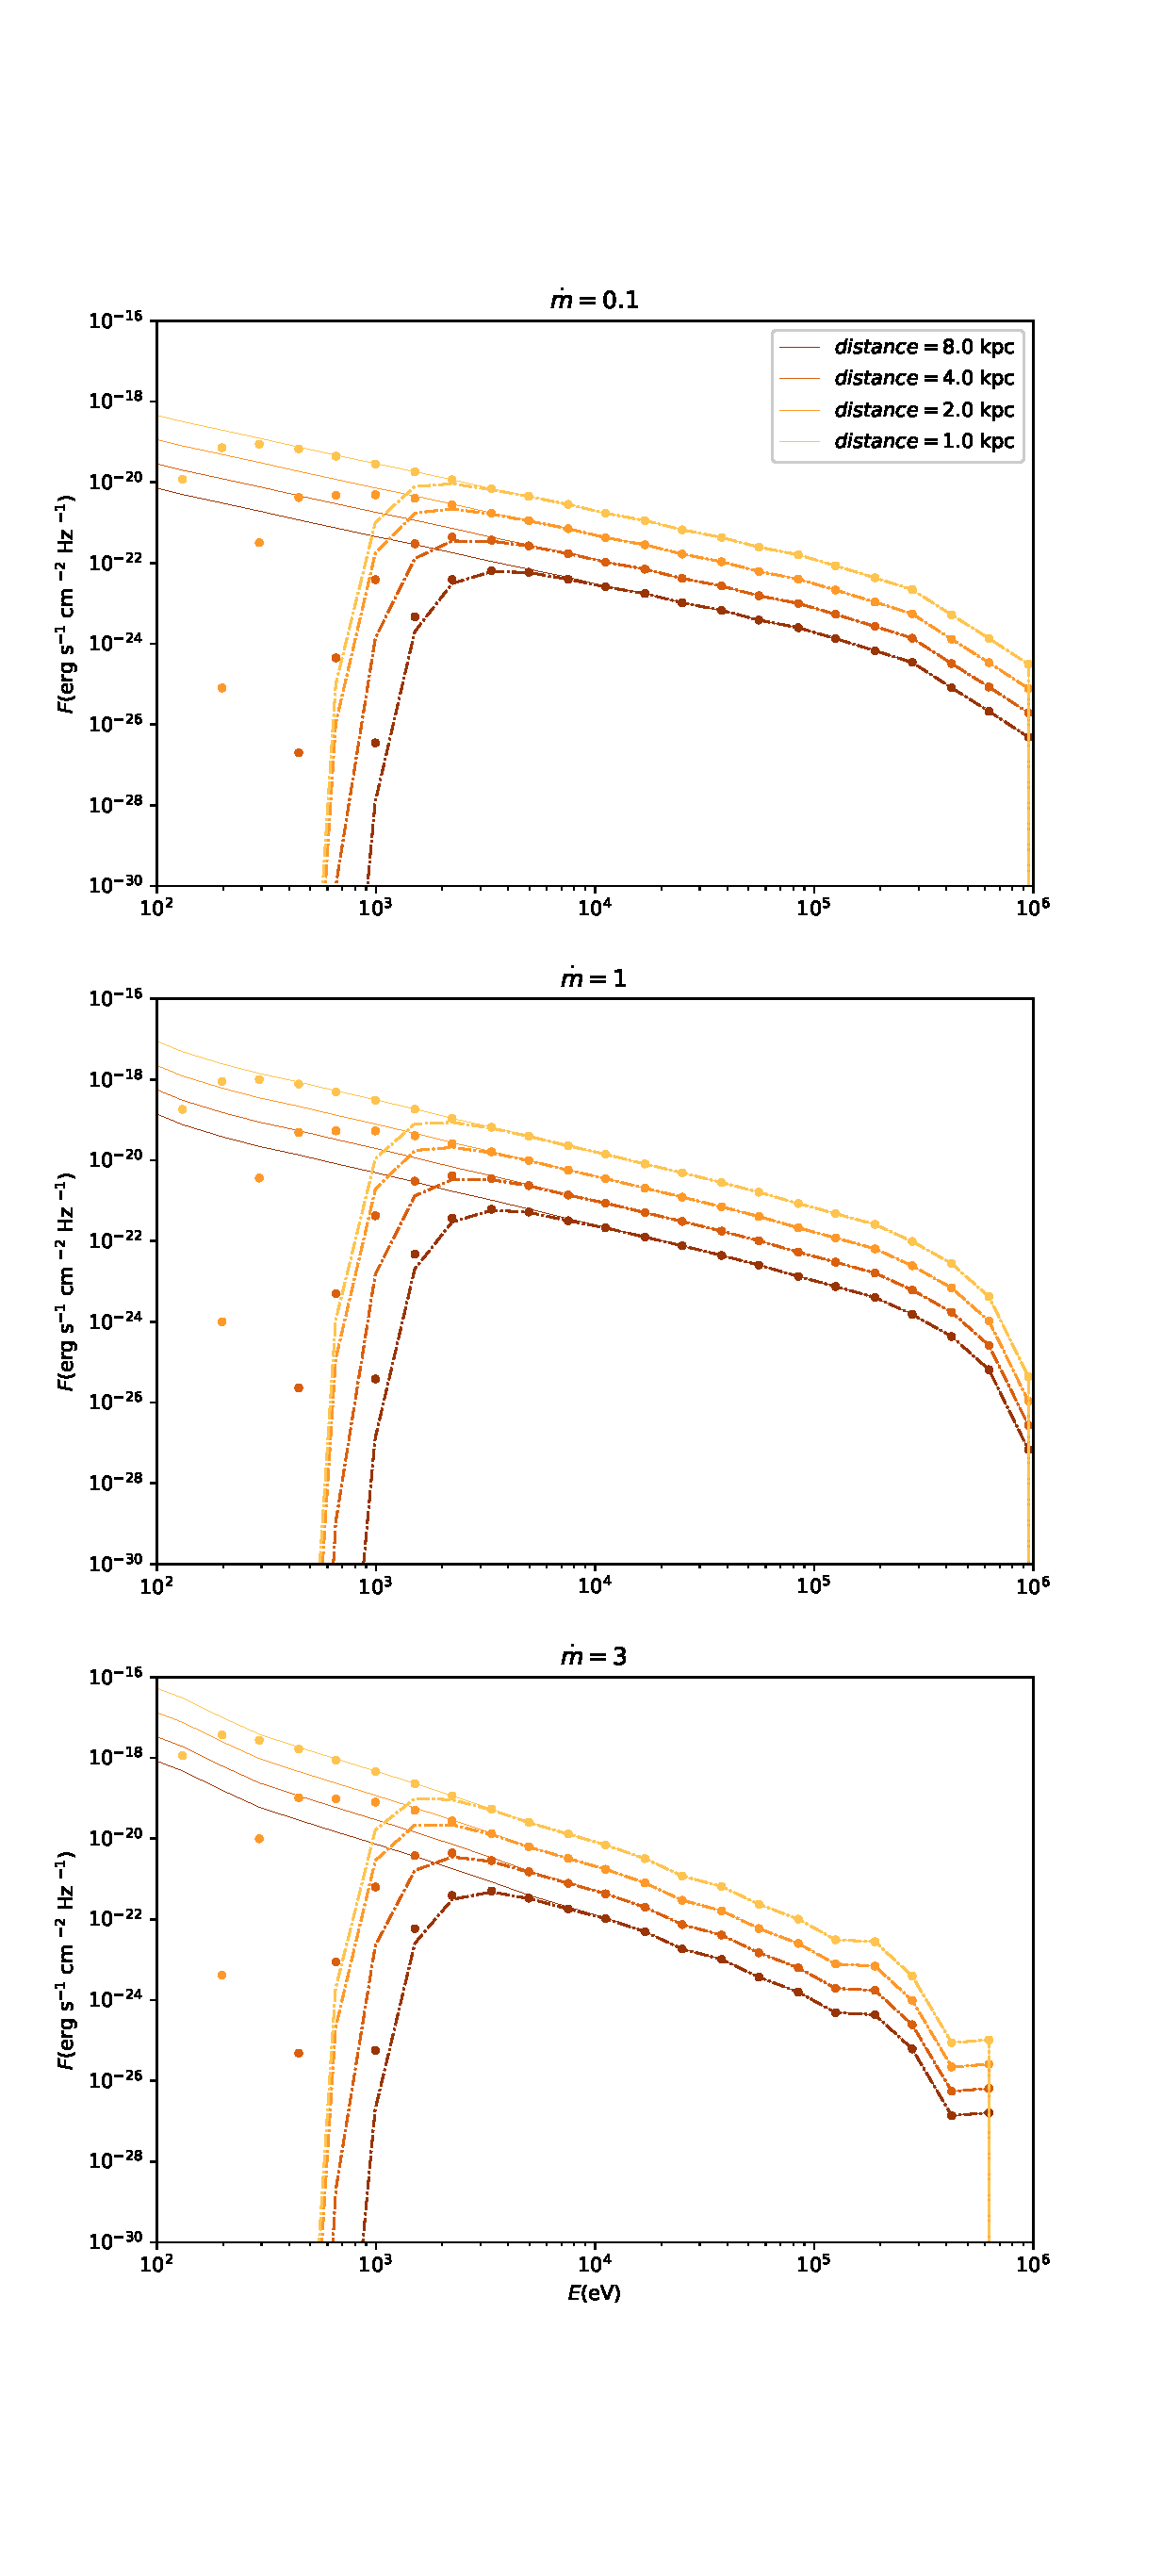
\includegraphics[width=0.5\textwidth]{2_2_1_1.eps}
	\caption{Monochromatic flux of X-ray at different distance (1, 2, 4, 8 kpc) from the galactic center. Darker color corresponds to larger galactic distance. Different accretion rates (0.1, 1 and 3 times the Eddington accretion rate) are utilized in three models, respectively, while other parameters of the AGN are taken to be $\alpha=0.1$ and $\beta=100$. The solid lines correspond to the primal monochromatic fluxes, the dots include the galactic absorption, while the dash-dotted lines show the fluxes which reach the center of the dense cloud where the total number density of hydrogen $n_{\ce{H}}=2\times10^4\text{ cm}^{-3}$.}
\end{figure}
	\subsubsection{Secondary ionization}
	All chemical species undergo direct X-ray ionization, while most of the primary electrons in a dense cloud are emitted during the primary ionization of $\ce{H}$ (mostly in hydrogen molecules) and $\ce{He}$ because of their high abundances. These rapid electrons collide with atoms to ionize them, which is known as secondary ionization, whose rate can be given as \citep{Maloney1996, Stauber2005}
	$$
	\zeta^i_{sec}=\int_{E_{min}}^{E_{max}}\frac{F(E)}{E}N_{sec}(E,x_e)\sigma^i_e(E)\text{d}E
	$$
	where $N_{sec}(E,x_e)$ is the number of secondary ionization events produced by one secondary electron, which can be expressed with the energy of the photoelectron ($E$), the ionization threshold of the atom ($E_{th}$), the mean energy expended to produce an ion pair through rapid electron process ($W$) and the fraction of energy of the photoelectron going into ionization $\eta$ :
	$$
	N_{sec}(E,x_e)=\frac{\eta E-E_{th}}{W(E)}
	$$
	In cold dense clouds illuminated by hard X-ray photons ($h\nu\gtrsim1\text{ keV}$), secondary ionization dominates because for $x_e\le1\%$, approximately $40\%$ of the energy of primary photoelectrons goes to ionization. For the ground state of neutral $\ce{H}$ with a ionization threshold $E_{th}=13.6\text{ eV}$. By taking $\eta=40\%$ and $W(E)=E_{th}$ we have $N_{sec}(E,x_e)\approx30\gg1$. 
	\subsection{Cosmic-ray chemistry}
	\subsection{Chemical networks}
	
	\section{Models}
	\subsection{X-ray models}
	\subsection{Molecular cloud models}
	Pseudo-time-dependent approach
	KROME package\footnote{\url{http://kromepackage.org/}} \citep{Grassi2014}
	
	\section{Results}
	
	\section{Discussions}
	\bibliography{ack.bib}

	
\end{document}
